\setlength{\imagewidth}{0.49\linewidth}%
\newdimen\imypos
\imypos=1.1\imagewidth
\begin{tikzpicture}[%
	img/.style={anchor=north west, inner sep=0},%
	txt/.style={font=\normalsize, inner sep=2pt, anchor=south west}%
	]%
	%
	\begin{scope}
	\clip(0,-0.15\imagewidth) rectangle (2\imagewidth, -2\imagewidth);
	\node[img] (im1) at (          0,         0) {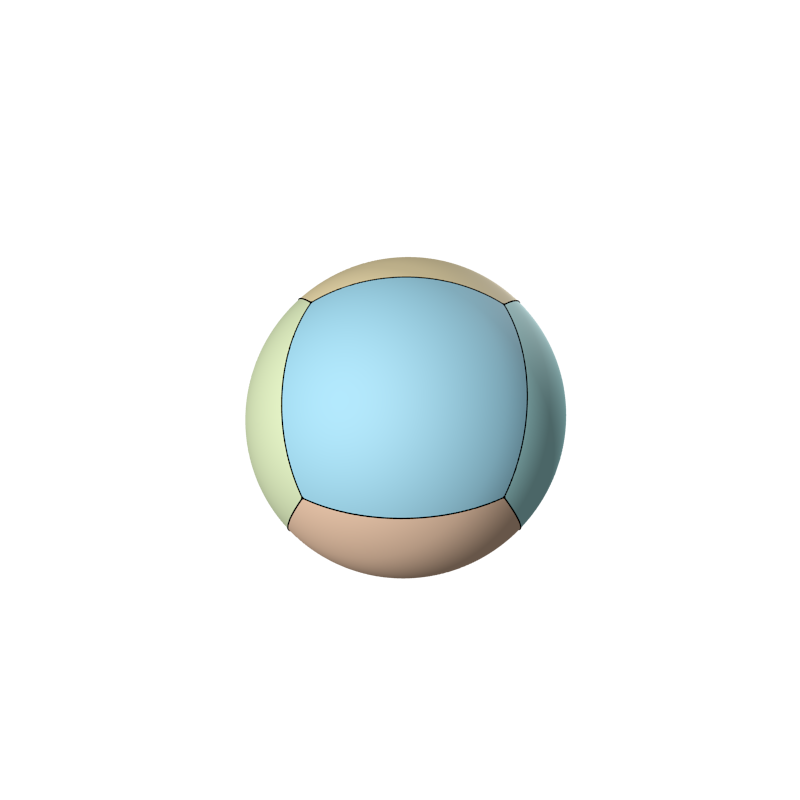
\includegraphics[width=\imagewidth]{vortex/snap_001}};
	\node[img] (im2) at (\imagewidth,         0) {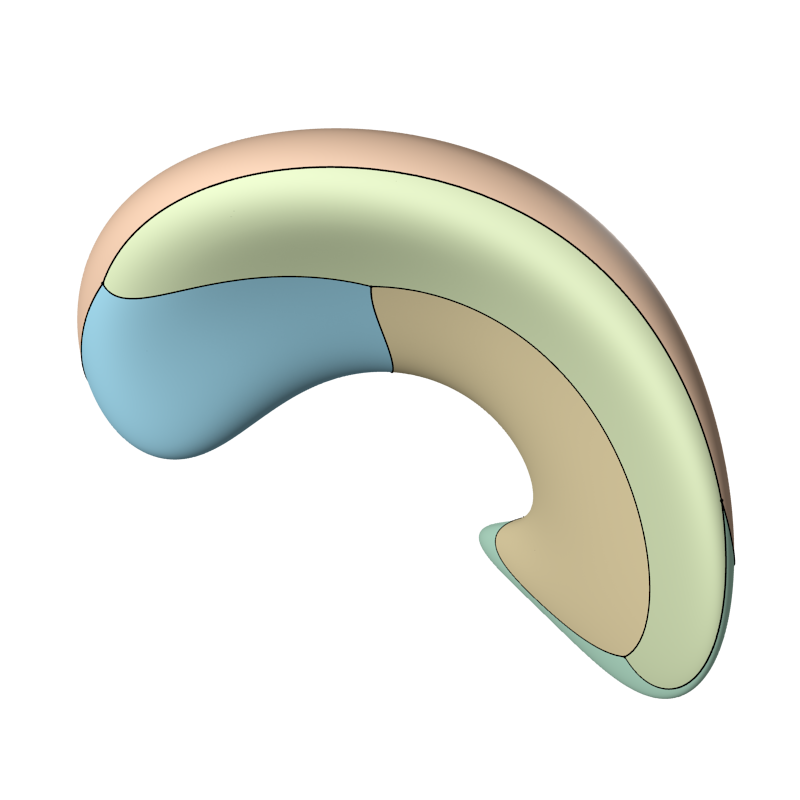
\includegraphics[width=\imagewidth]{vortex/snap_002}};
	\end{scope}
	\node[img] (im3) at (          0,  -\imypos) {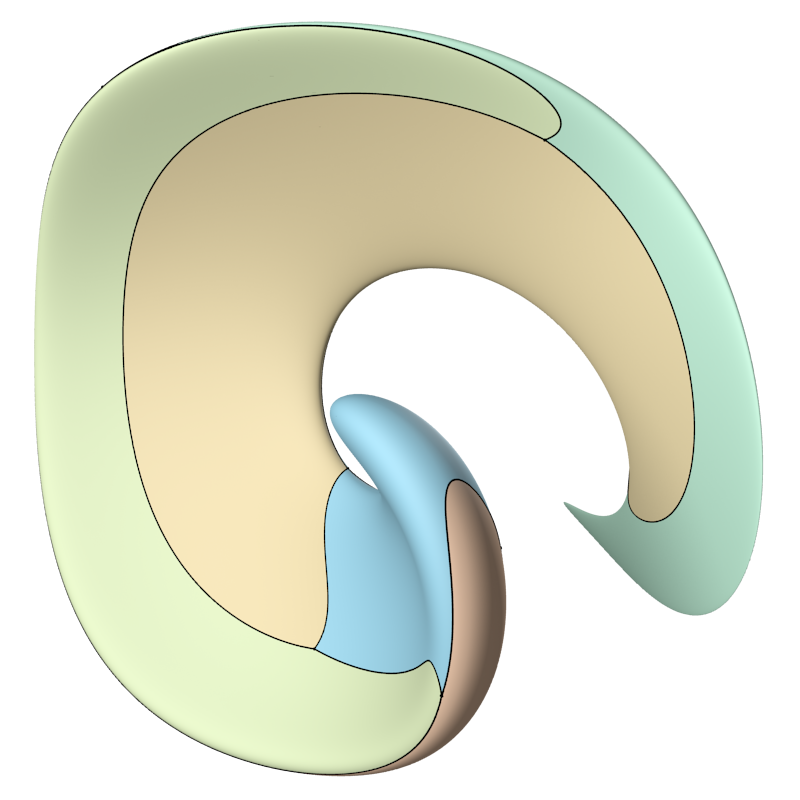
\includegraphics[width=\imagewidth]{vortex/snap_003}};
	\node[img] (im4) at (\imagewidth,  -\imypos) {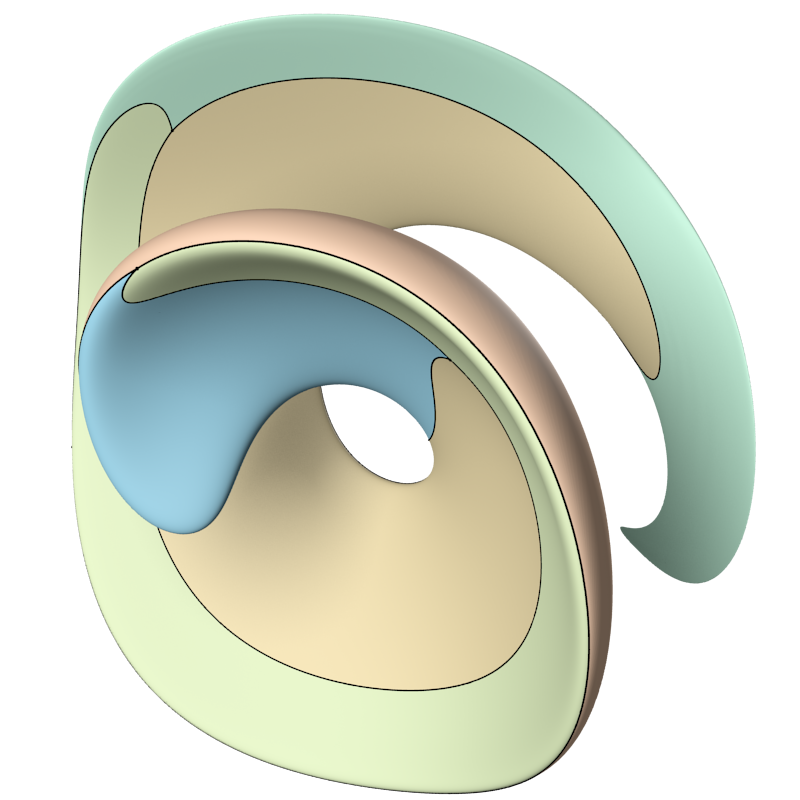
\includegraphics[width=\imagewidth]{vortex/snap_004}};
	\node[img] (im5) at (          0, -2\imypos) {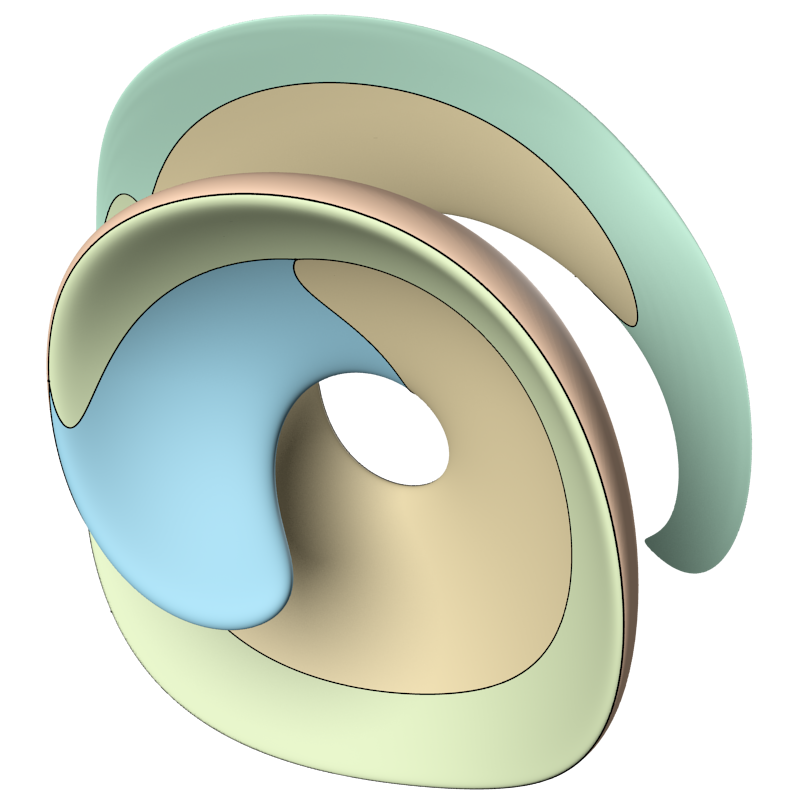
\includegraphics[width=\imagewidth]{vortex/snap_005}};
	\node[img] (im6) at (\imagewidth, -2\imypos) {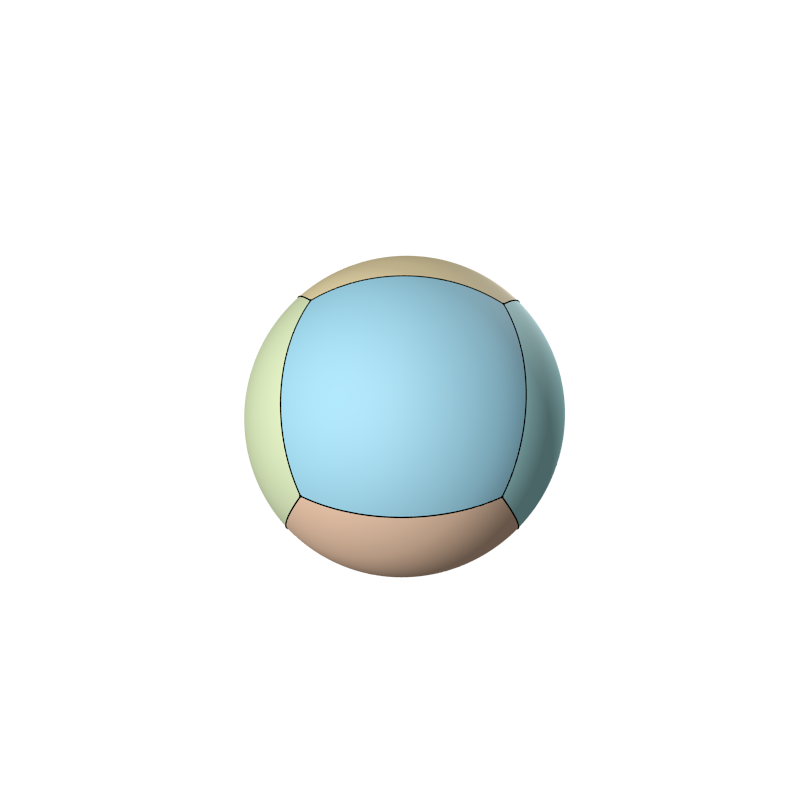
\includegraphics[width=\imagewidth]{vortex/snap_006}};
	%
	\node[txt] at (im1.south west) {$t=   0$};
    \node[txt] at (im2.south west) {$t= T/8$};
    \node[txt] at (im3.south west) {$t= T/4$};
    \node[txt] at (im4.south west) {$t=3T/8$};
    \node[txt] at (im5.south west) {$t= T/2$};
    \node[txt] at (im6.south west) {$t=   T$};
\end{tikzpicture}